% !TeX spellcheck = ug_CN-China
\documentclass[UTF8,12pt,AutoFakeBold]{ctexart}
%广西大学物理学院2021级硕士王信哲制作
%加载并设置宏包
%广西大学物理学院2021级硕士王信哲制作
\ctexset{
	bibname = 参考文献,
	contentsname=\heiti\zihao{3} 目\ 录,
	section={
		name={第,章},number=\chinese{section},
		format=\heiti\bfseries\centering\zihao{3}\linespread{1.25},
		beforeskip=20pt,%18ex plus 0.2ex minus .2ex,
		afterskip=20pt%18ex plus 0.2ex minus .2ex
	},
	subsection={
		format=\heiti\bfseries\raggedright\zihao{4}\linespread{1.25},
		beforeskip=8.75pt,%18ex plus 0.1ex minus .1ex,
		afterskip=8.75pt%18ex plus 0.1ex minus .1ex
	},
	subsubsection={
		format=\heiti\bfseries\raggedright\zihao{-4}\linespread{1.25},
		beforeskip=0pt,
		afterskip=0pt
	},
	appendix/name=附录
}
%\usepackage{ctex}%設置中文

\usepackage{tocloft}
\renewcommand{\cfttoctitlefont}{\hfill} % 将目录标题设置为三号字、黑体
\renewcommand{\cftaftertoctitle}{\hfill} % 将目录标题居中
\renewcommand{\cftsecleader}{\cftdotfill{\cftdotsep}}%让一级标题的章节和页面之间也有点线连接
\renewcommand{\cftsecfont}{\normalfont}%取消section字体在目录中加粗
\renewcommand{\cftsecpagefont}{\normalfont}%取消section在目录中对应的页码加粗
\setlength{\cftbeforesecskip}{0pt}
\renewcommand{\cftdotsep}{1}


\setCJKmainfont{宋体}%设置全局中文字体
\usepackage{fontspec}%设置英文
\setmainfont{Times New Roman} % 设置英文为Times New Roman
\usepackage{amsmath,amssymb,amsthm}
\let\hbaroriginal\hbar
\AtBeginDocument{\let\hbar\hbaroriginal}
%\usepackage{unicode-math}
%\setmathfont{Latin Modern Math}

\usepackage{geometry}
\geometry{papersize={21cm,29.7cm}}
\geometry{left=2.8cm,right=2.5cm,top=2.8cm,bottom=2.2cm}
\usepackage{mathrsfs}
\usepackage{wasysym}
\usepackage{braket}
\usepackage{indentfirst}
\usepackage{cases}
\usepackage{bm}
\usepackage{graphicx}
\usepackage{subcaption}
\usepackage{longtable,booktabs}
\usepackage{color}
\usepackage[colorlinks,linkcolor=blue,anchorcolor=blue,citecolor=blue]{hyperref}%#006eb2
%\hypersetup{
	%	colorlinks=true,
	%	linkcolor=[rgb]{0,0.43,0.70},
	%	citecolor=[rgb]{0,0.43,0.70},
	%	filecolor=[rgb]{0,0.43,0.70},
	%	urlcolor=[rgb]{0,0.43,0.70}
	%}
\usepackage{cleveref}   %可以调用 \Cref{fig:xxx}或者 \ref{fig:xxx}
\usepackage{pdfpages}
\usepackage{float}
\usepackage{booktabs}
\usepackage{fancyhdr}%設置頁眉

\usepackage{setspace}%设置行间距
\setstretch{1.25}

\usepackage[nottoc]{tocbibind}%[nottoc,numbib]
%\usepackage{gbt7714}
\usepackage{gbt7714-gxu}
\bibliographystyle{gxu}
\usepackage{natbib}
\setlength{\bibsep}{0pt}
%\bibliographystyle{gbt7714-numerical}

\usepackage{appendix}


\usepackage{booktabs}
\usepackage{lipsum} % 用于生成随机文本
\graphicspath{{图/}{./}}
\usepackage[justification=centering]{caption}
\usepackage{bicaption}
\captionsetup[figure][bi]{labelfont=bf, textfont=bf}
\captionsetup[figure][bi-second]{name=Figure,labelfont=bf,textfont=bf}
\captionsetup[table][bi]{labelfont=bf, textfont=bf}
\captionsetup[table][bi-second]{name=Table,labelfont=bf,textfont=bf}

%设置图表编号格式为{章节号}-{章节内序号}
\usepackage{chngcntr}
\counterwithin{figure}{section}
\counterwithin{table}{section}
\renewcommand{\thefigure}{\thesection-\arabic{figure}}
\renewcommand{\thetable}{\thesection-\arabic{table}}

\usepackage{pdfpages}

% 定义中文摘要环境
\newenvironment{cnabstract}{
	\par\small
	\noindent\mbox{}\hfill{\bfseries \cnabstractname}\hfill\mbox{}
	\par\vskip 2.5ex
}{\par\vskip 2.5ex}

% 定义英文摘要环境
\newenvironment{enabstract}{
	\par\small
	\noindent\mbox{}\hfill{\bfseries \enabstractname}\hfill\mbox{}
	\par\vskip 2.5ex
}{\par\vskip 2.5ex}

\newcommand{\cnabstractname}{\heiti \fontsize{16pt}{20pt}\textbf{摘\ 要}} % 中文摘要标题
\newcommand{\enabstractname}{\fontsize{16pt}{20pt}\textbf{ABSTRACT}} % 英文摘要标题


\begin{document}
	%加载封面;封面需要自己修改word模板后导出为pdf文件---------------------------------------------------
	\setcounter{page}{1} % 重置页码
	\pagenumbering{roman}
	\includepdf[pages={-}]{毕业论文封面.pdf}
	
	
	%设置摘要、目录部分页码------------------------------------------------------------------------------
	\setcounter{page}{1} % 重置页码
	\pagenumbering{Roman}
	\pagestyle{fancy}%清除原页眉页脚样式
	\fancyhf{}
	\fancyfoot[C]{\thepage} % 在页脚中间添加页码
	
	
	%摘要部分--------------------------------------------------------------------------------------------
	\section*{论文中文标题}
	\begin{cnabstract}\addcontentsline{toc}{section}{摘\ 要}
		\fontsize{14pt}{17.5pt}\selectfont%设置字体为四号,行间距1.25倍
		\textcolor{red}{毕业论文封面请自己复制学校的word模板修改后导出为pdf格式,并命名为毕业论文封面.pdf覆盖本文件夹中同名文件。封面的格式可能学校会修改,所以务必自行检查!}
		\par
		摘要是论文内容的总结概括,摘要内容一般应包含研究工作的目的、研究方法、结果和最终结论等,重点突出具有创新性的成果和新见解。不宜使用公式、图表,不标注引用文献。硕士论文摘要一般为500到800字,不宜超过1000字。博士论文摘要一般为1000到1500字,不宜超过2000字。关键词应体现论文特色,具有语义性,在论文中有明确的出处。并应尽量采用《汉语主题词表》或各专业主题词表提供的规范词。一般列出3到8个关键词。英文摘要及关键词应与中文摘要内容、关键词相对应。
		\par
		论文题目为三号黑体字居中打印;“摘要”二字与题目空一行,为三号黑体,字间空一格;摘要内容为四号宋体,每段开头空二格,标点符号占一格;“关键词”与摘要内容空一行,四号黑体,其后为关键词(四号宋体)。关键词之间用两个空格分开,最后一个关键词后不打标点符号。
		英文摘要的字号与中文摘要相同。题目全部采用大写字母,居中打印。每行左右两边至少留五个字符空格。“ABSTRACT”与题目空一行居中打印,再下,空一行打印英文摘要内容;摘要内容每段开头留四个字符空格;摘要内容后,下空二行打印“KEY WORDS”,其后关键词首字母大写,每一关键词之间用分号隔开,最后一个关键词后不打标点符号。全文英文一律采用“Times New Roman”字体。
		\\
		\\
		\heiti 关键词:
		\songti 关键词1\ \ 关键词2\ \ 关键词3\ \ 关键词4\ \ 关键词5
	\end{cnabstract}
	\pagebreak
	\section*{CAPITALISING THE ENGLISH TITLE OF A DISSERTATION}
	\begin{enabstract}\addcontentsline{toc}{section}{ABSTRACT}
		\fontsize{14pt}{17.5pt}\selectfont%设置字体为四号,行间距1.25倍
		
		Abstract is a summary of the content of the paper, the abstract content should generally contain the purpose of the research work, research methodology, results and final conclusions, etc., focusing on innovative results and new insights. It is not appropriate to use formulas, charts and diagrams, and cited literature is not marked. The abstract of master's thesis is generally 500 to 800 words, and should not exceed 1,000 words. The abstract of doctoral dissertation should be 1000 to 1500 words, not more than 2000 words. Keywords should reflect the characteristics of the dissertation, be semantic, and have a clear source in the dissertation. And they should try to adopt the standard words provided by the Chinese Theme Word List or the theme word lists of each speciality. Generally 3 to 8 keywords are listed. The English abstract and keywords should correspond to the content of the Chinese abstract and keywords.
		\par
		The title of the paper is printed in three-pointed boldface in the centre; "Abstract" and the title of the two words in an empty line, for the three-pointed boldface, the word between the empty space; the abstract content for the four-pointed Song, the beginning of each paragraph empty space, punctuation marks account for a space; "Keywords" and the content of the abstract in an empty line, the four-pointed Keywords" and the abstract content of an empty line, four bold, followed by the key words (four Song). The keywords are separated by two spaces, and the last keyword is not punctuated.
		The font size of the English abstract is the same as that of the Chinese abstract. The title should be printed in all capital letters and centred. Leave at least five character spaces on the left and right sides of each line. "ABSTRACT" and the title of an empty line in the centre of the print, and then under, an empty line to print the content of the English summary; summary of the content of the beginning of each paragraph to stay four characters space; summary of the content, the next two lines of the empty print "KEY WORDS", and then the keywords The first letter is capitalised, each keyword is separated by a semicolon, and the last keyword is not punctuated. The whole text in English is in "Times New Roman" font.
		\\
		\\
		\textbf{KEW WORDS:} KEW WORDS 1;  KEW WORDS 2;  KEW WORDS 3;  KEW WORDS 4;  KEW WORDS 5
	\end{enabstract}
	\pagebreak
	%摘要---------------------------------------------------------------------------
	
	
	{\hypersetup{colorlinks=true,linkcolor=black}\tableofcontents}
	\newpage
	\setcounter{page}{1} % 重置页码
	\pagenumbering{arabic} % 开始阿拉伯数字编码
	%R:页面右边%L:页面左边%C:页面中间
	\pagestyle{fancy}%清除原页眉页脚样式
	\fancyhf{}
	\fancyhead[L]{\lishu \fontsize{12pt}{15pt}\selectfont 广西大学硕士学位论文}%\leftmark:表示“一级标题”
%	\fancyhead[C]{\rightmark}%\rightmark:表示“二级标题”
	\fancyhead[R]{\lishu \fontsize{12pt}{15pt}\selectfont 宇宙磁单极子疑难的原初黑洞吸积解}%\thepage:表示“页码”
	\fancyfoot[C]{\thepage} % 在页脚中间添加页码
	\section{绪论\label{绪论}}
	这是一个符合广西大学要求的模板,为了给出一些具体格式的实例,下文将会随机给出一些文字、公式、表格、图片和引用\cite{doi:10.1080/00107514.2012.685693,annurev:/content/journals/10.1146/annurev-nucl-102014-022137,GROOM1986323,doi:10.1142/S0217751X20300124}。
	\par
	黄帝者,少典之子,姓公孙,名曰轩辕。生而神灵,弱而能言,幼而徇齐,长而敦敏,成而聪明\cite{HOOFT1974276,PismaZhETF.20.430}。
	\par
	轩辕之时,神农氏世衰。诸侯相侵伐,暴虐百姓,而神农氏弗能征。于是轩辕乃习用干戈,以征不享,诸侯咸来宾从。而蚩尤最为暴,莫能伐。炎帝欲侵陵诸侯,诸侯咸归轩辕。轩辕乃修德振兵,治五气,蓺五种,抚万民,度四方,教熊罴貔貅貙虎,以与炎帝战于阪泉之野。三战,然后得其志。蚩尤作乱,不用帝命。于是黄帝乃征师诸侯,与蚩尤战于涿鹿之野,遂禽杀蚩尤。而诸侯咸尊轩辕为天子\cite{PhysRevLett.33.451},代神农氏,是为黄帝。天下有不顺者,黄帝从而征之,平者去之,披山通道,未尝宁居。
	东至于海,登丸山,及岱宗。西至于空桐,登鸡头。南至于江,登熊、湘。北逐荤粥,合符釜山,而邑于涿鹿之阿。迁徙往来无常处,以师兵为营卫。官名皆以云命,为云师。置左右大监,监于万国。万国和,而鬼神山川封禅与为多焉。获宝鼎,迎日推策。举风后、力牧、常先、大鸿以治民。顺天地之纪,幽明之占,死生之说,存亡之难。时播百谷草木,淳化鸟兽虫蛾,旁罗日月星辰水波土石金玉,劳勤心力耳目,节用水火材物。有土德之瑞,故号黄帝。
	\par
	黄帝二十五子,其得姓者十四人。
	黄帝居轩辕之丘,而娶于西陵之女,是为嫘祖。嫘祖为黄帝正妃,生二子,其后皆有天下:其一曰玄嚣,是为青阳\cite{STAROBINSKY198099,PhysRevD.23.347},青阳降居江水;其二曰昌意,降居若水。昌意娶蜀山氏女,曰昌仆,生高阳,高阳有圣德焉。黄帝崩,葬桥山。其孙昌意之子高阳立,是为帝颛顼也。
	\par
	帝颛顼高阳者,黄帝之孙而昌意之子也。静渊以有谋,疏通而知事;养材以任地,载时以象天,依鬼神以制义,治气以教化,絜诚以祭祀。北至于幽陵,南至于交趾,西至于流沙,东至于蟠木。动静之物,大小之神,日月所照,莫不砥属。
	帝颛顼生子曰穷蝉。颛顼崩,而玄嚣之孙高辛立,是为帝喾。
	\par
	帝喾高辛者,黄帝之曾孙也。高辛父曰蟜极,蟜极父曰玄嚣,玄嚣父曰黄帝。自玄嚣与蟜极皆不得在位,至高辛即帝位。高辛于颛顼为族子。
	\par
	高辛生而神灵,自言其名。普施利物,不于其身。聪以知远,明以察微。顺天之义,知民之急。仁而威,惠而信,修身而天下服。取地之财而节用之,抚教万民而利诲之,历日月而迎送之,明鬼神而敬事之。其色郁郁,其德嶷嶷。其动也时,其服也士。帝喾溉执中而遍天下,日月所照,风雨所至,莫不从服。
	帝喾娶陈锋氏女,生放勋。娶娵訾氏女,生挚。帝喾崩,而挚代立。帝挚立,不善,而弟放勋立,是为帝尧。
	\par
	帝尧者,放勋。其仁如天,其知如神。就之如日,望之如云。富而不骄,贵而不舒。黄收纯衣,彤车乘白马。能明驯德,以亲九族。九族既睦,便章百姓。百姓昭明,合和万国。
	乃命羲、和,敬顺昊天,数法日月星辰,敬授民时。分命羲仲,居郁夷,曰旸谷。敬道日出,便程东作。日中,星鸟,以殷中春。其民析,鸟兽字微。申命羲叔,居南交。便程南讹,敬致。日永,星火,以正中夏。其民因,鸟兽希革。申命和仲,居西土,曰昧谷。敬道日入,便程西成。夜中,星虚,以正中秋。其民夷易,鸟兽毛毨。申命和叔;居北方,曰幽都。便在伏物。日短,星昴,以正中冬。其民燠,鸟兽氄毛。岁三百六十六日,以闰月正四时。信饬百官,众功皆兴。
	尧曰:“谁可顺此事?”放齐曰:“嗣子丹朱开明。”尧曰:“吁!顽凶,不用。”尧又曰:“谁可者?”讙兜曰:“共工旁聚布功,可用。”尧曰:“共工善言,其用僻,似恭漫天,不可。”尧又曰:“嗟,四岳,汤汤洪水滔天,浩浩怀山襄陵,下民其忧,有能使治者?”皆曰鲧可。尧曰:“鲧负命毁族,不可。”岳曰:“异哉,试不可用而已。”尧于是听岳用鲧。九岁,功用不成。
	尧曰:“嗟!四岳:朕在位七十载,汝能庸命,践朕位?”岳应曰:“鄙德忝帝位。”尧曰:“悉举贵戚及疏远隐匿者。”众皆言于尧曰:“有矜在民间,曰虞舜。”尧曰:“然,朕闻之。其何如?”岳曰:“盲者子。父顽,母嚚,弟傲,能和以孝,烝烝治,不至奸。”尧曰:“吾其试哉。”于是尧妻之二女,观其德于二女。舜饬下二女于妫汭,如妇礼。尧善之,乃使舜慎和五典,五典能从。乃遍入百官,百官时序。宾于四门,四门穆穆,诸侯远方宾客皆敬。尧使舜入山林川泽,暴风雷雨,舜行不迷。尧以为圣,召舜曰:“女谋事至而言可绩,三年矣。女登帝位。”舜让于德不怿。正月上日,舜受终于文祖。文祖者,尧大祖也。
	\par
	于是帝尧老,命舜摄行天子之政,以观天命。舜乃在璿玑玉衡,以齐七政。遂类于上帝,禋于六宗,望于山川,辩于群神。揖五瑞,择吉月日,见四岳诸牧,班瑞。岁二月,东巡狩,至于岱宗,祡,望秩于山川。遂见东方君长,合时月正日,同律度量衡,修五礼五玉三帛二生一死为挚,如五器,卒乃复。五月,南巡狩;八月,西巡狩;十一月,北巡狩:皆如初。归,至于祖祢庙,用特牛礼。五岁一巡狩,群后四朝。遍告以言,明试以功,车服以庸。肇十有二州,决川。象以典刑,流宥五刑,鞭作官刑,扑作教刑,金作赎刑。眚灾过,赦;怙终贼,刑。钦哉,钦哉,惟刑之静哉!
	讙兜进言共工,尧曰不可而试之工师,共工果淫辟。四岳举鲧治鸿水,尧以为不可,岳彊请试之,试之而无功,故百姓不便。三苗在江淮、荆州数为乱。于是舜归而言于帝,请流共工于幽陵,以变北狄;放驩兜于崇山,以变南蛮;迁三苗于三危,以变西戎;殛鲧于羽山,以变东夷:四罪而天下咸服。
	\par
	尧立七十年得舜,二十年而老,令舜摄行天子之政,荐之于天。尧辟位凡二十八年而崩。百姓悲哀,如丧父母。三年,四方莫举乐,以思尧。尧之子丹朱之不肖,不足授天下,于是乃权授舜。授舜,则天下得其利而丹朱病;授丹朱,则天下病而丹朱得其利。尧曰“终不以天下之病而利一人”,而卒授舜以天下。尧崩,三年之丧毕,舜让辟丹朱于南河之南。诸侯朝觐者不之丹朱而之舜,狱讼者不之丹朱而之舜,讴歌者不讴歌丹朱而讴歌舜。舜曰“天也”,夫而后之中国践天子位焉,是为帝舜。
	\par
	虞舜者,名曰重华。重华父曰瞽叟,瞽叟父曰桥牛,桥牛父曰句望,句望父曰敬康,敬康父曰穷蝉,穷蝉父曰帝颛顼,颛顼父曰昌意:以至舜七世矣。自从穷蝉以至帝舜,皆微为庶人。
	舜父瞽叟盲,而舜母死,瞽叟更娶妻而生象,象傲。瞽叟爱后妻子,常欲杀舜,舜避逃;及有小过,则受罪。舜事父及后母与弟,日以笃谨,匪有解。
	\par
	舜,冀州之人也。舜耕历山,渔雷泽,陶河滨,作什器于寿丘,就时于负夏。舜父瞽叟顽,母嚚,弟象傲,皆欲杀舜。舜顺适不失子道,兄弟孝慈。欲杀,不可得;即求,尝在侧。
	舜年二十以孝闻。三十而帝尧问可用者,四岳咸荐虞舜,曰可。于是尧乃以二女妻舜以观其内,使九男与处以观其外。舜居妫汭,内行弥谨。尧二女不敢以贵骄事舜亲戚,甚有妇道。尧九男皆益笃。舜耕历山,历山之人皆让畔;渔雷泽,雷泽上人皆让居;陶河滨,河滨器皆不苦窳。一年而所居成聚,二年成邑,三年成都。尧乃赐舜絺衣,与琴,为筑仓廪,予牛羊。瞽叟尚复欲杀之,使舜上涂廪,瞽叟从下纵火焚廪。舜乃以两笠自扞而下,去,得不死。后瞽叟又使舜穿井,舜穿井为匿空旁出。舜既入深,瞽叟与象共下土实井,舜从匿空出,去。瞽叟、象喜,以舜为已死。象曰“本谋者象。”象与其父母分,于是曰:“舜妻尧二女,与琴,象取之。牛羊仓廪予父母。”象乃止舜宫居,鼓其琴。舜往见之。象鄂不怿,曰:“我思舜正郁陶!”舜曰:“然,尔其庶矣!”舜复事瞽叟爱弟弥谨。于是尧乃试舜五典百官,皆治。
	\par
	昔高阳氏有才子八人,世得其利,谓之“八恺”。高辛氏有才子八人,世谓之“八元”。此十六族者,世济其美,不陨其名。至于尧,尧未能举。舜举八恺,使主后土,以揆百事,莫不时序。举八元,使布五教于四方,父义,母慈,兄友,弟恭,子孝,内平外成。
	昔帝鸿氏有不才子,掩义隐贼,好行凶慝,天下谓之浑沌。少暤氏有不才子,毁信恶忠,崇饰恶言,天下谓之穷奇。颛顼氏有不才子,不可教训,不知话言,天下谓之檮杌。此三族世忧之。至于尧,尧未能去。缙云氏有不才子,贪于饮食,冒于货贿,天下谓之饕餮。天下恶之,比之三凶。舜宾于四门,乃流四凶族,迁于四裔,以御螭魅,于是四门辟,言毋凶人也。
	
	
	\newpage
	
	\section{一级标题\label{章节:正文部分}}
	\subsection{二级标题1\label{章节:二级标题1}}
	
	
	以下是一些公式的示例\footnote{这是一个脚注的示例}:
	\begin{equation}
		\frac{\hbar c}{e^2}=137
	\end{equation}
	\begin{subnumcases}{\label{式:绪论|对称的麦克斯韦方程组}}
		\text{d}^*\!\bm{F}=4\pi^*\!\!\bm{J}\\
		\text{d}\bm{F}=4\pi^*\!\!\hat{\bm{J}}
	\end{subnumcases}
	其中电磁场$\bm{F}$为四维流形上的二形式场,电流密度$\bm{J}$和磁流密度$\hat{\bm{J}}$为三形式场,$^*\!\bm{F}$是$\bm{F}$的对偶形式,$^*\!\!\bm{J}$和$^*\!\!\hat{\bm{J}}$同理。
	\par
	下面继续随便放些文字上去,引用是随便写的,仅仅是示例。
	\par
	舜入于大麓,烈风雷雨不迷\cite{HOOFT1974276,PismaZhETF.20.430},尧乃知舜之足授天下。尧老,使舜摄行天子政,巡狩。舜得举用事二十年,而尧使摄政。摄政八年而尧崩\cite{1975CMaPh..43..199H}。三年丧毕,让丹朱,天下归舜。而禹、皋陶、契、后稷、伯夷、夔、龙、倕、益、彭祖自尧时而皆举用,未有分职。于是舜乃至于文祖,谋于四岳,辟四门,明通四方耳目,命十二牧论帝德,行厚德,远佞人,则蛮夷率服。舜谓四岳曰:“有能奋庸美尧之事者,使居官相事?”皆曰:“伯禹为司空,可美帝功。”舜曰:“嗟,然!禹,汝平水土,维是勉哉。”禹拜稽首,让于稷、契与皋陶。舜曰:“然,往矣。”舜曰:“弃,黎民始饥,汝后稷播时百谷。”舜曰:“契,百姓不亲,五品不驯,汝为司徒\cite{PhysRevLett.43.1365,ZELDOVICH1978239,Weinberg_2012},而敬敷五教,在宽。”舜曰:“皋陶,蛮夷猾夏,寇贼奸轨,汝作士,五刑有服,五服三就;五流有度,五度三居:维明能信。”舜曰:“谁能驯予工?”皆曰垂可。于是以垂为共工。舜曰:“谁能驯予上下草木鸟兽?”皆曰益可。于是以益为朕虞。益拜稽首,让于诸臣朱虎、熊罴。舜曰:“往矣,汝谐。”遂以朱虎、熊罴为佐。舜曰:“嗟!四岳,有能典朕三礼?”皆曰伯夷可。舜曰:“嗟!伯夷,以汝为秩宗,夙夜维敬,直哉维静絜。”伯夷让夔、龙。舜曰:“然。以夔为典乐,教稺子,直而温,宽而栗,刚而毋虐,简而毋傲;诗言意,歌长言,声依永,律和声,八音能谐,毋相夺伦,神人以和。”夔曰:“于!予击石拊石,百兽率舞。”舜曰:“龙,朕畏忌谗说殄伪,振惊朕众,命汝为纳言,夙夜出入朕命,惟信。”舜曰:“嗟!女二十有二人,敬哉,惟时相天事。”三岁一考功,三考绌陟,远近众功咸兴。分北三苗。
	此二十二人咸成厥功:皋陶为大理,平,民各伏得其实;伯夷主礼,上下咸让;垂主工师,百工致功;益主虞,山泽辟;弃主稷,百谷时茂;契主司徒,百姓亲和;龙主宾客,远人至;十二牧行而九州莫敢辟违;唯禹之功为大,披九山,通九泽,决九河,定九州,各以其职来贡,不失厥宜。方五千里,至于荒服。南抚交趾、北发,西戎、析枝、渠廋、氐、羌,北山戎、发、息慎,东长、鸟夷,四海之内咸戴帝舜之功。于是禹乃兴九招之乐,致异物,凤皇来翔。天下明德皆自虞帝始。
	\par
	舜年二十以孝闻,年三十尧举之,年五十摄行天子事,年五十八尧崩,年六十一代尧践帝位。践帝位三十九年,南巡狩,崩于苍梧之野。葬于江南九疑,是为零陵。舜之践帝位,载天子旗,往朝父瞽叟,夔夔唯谨,如子道。封弟象为诸侯。舜子商均亦不肖,舜乃豫荐禹于天。十七年而崩。三年丧毕,禹亦乃让舜子,如舜让尧子。诸侯归之,然后禹践天子位。尧子丹朱,舜子商均,皆有疆土,以奉先祀。服其服,礼乐如之\cite{PhysRevLett.43.1365}。以客见天子,天子弗臣,示不敢专也。
	\par
	自黄帝至舜、禹,皆同姓而异其国号,以章明德。故黄帝为有熊,帝颛顼为高阳,帝喾为高辛,帝尧为陶唐,帝舜为有虞。帝禹为夏后而别氏,姓姒氏。契为商,姓子氏。弃为周,姓姬氏。
	\par
	太史公曰:学者多称五帝,尚矣。然尚书独载尧以来;而百家言黄帝,其文不雅驯,荐绅先生难言之。孔子所传宰予问五帝德及帝系姓,儒者或不传。余尝西至空桐,北过涿鹿,东渐于海,南浮江淮矣,至长老皆各往往称黄帝、尧、舜之处,风教固殊焉,总之不离古文者近是。予观春秋、国语,其发明五帝德、帝系姓章矣,顾弟弗深考,其所表见皆不虚。书缺有间矣,其轶乃时时见于他说。非好学深思,心知其意,固难为浅见寡闻道也。余并论次,择其言尤雅者,故著为本纪书首。
	
	
	
	
	
	\subsection{二级标题2\label{章节:二级标题2}}
	
	\subsubsection{三级标题1\label{章节:三级标题1}}
	
	本部分将示例图片插入。仍然随便放点文字上去。
	
	夏禹,名曰文命。禹之父曰鲧,鲧之父曰帝颛顼,颛顼之父曰昌意,昌意之父曰黄帝。禹者,黄帝之玄孙而帝颛顼之孙也。禹之曾大父昌意及父鲧皆不得在帝位,为人臣。
	
	当帝尧之时,鸿水滔天,浩浩怀山襄陵,下民其忧。尧求能治水者,群臣四岳皆曰鲧可。尧曰:“鲧为人负命毁族,不可。”四岳曰:“等之未有贤于鲧者,愿帝试之。”于是尧听四岳,用鲧治水。九年而水不息,功用不成。于是帝尧乃求人,更得舜。舜登用,摄行天子之政,巡狩。行视鲧之治水无状,乃殛鲧于羽山以死。天下皆以舜之诛为是。于是舜举鲧子禹,而使续鲧之业。
	
	尧崩,帝舜问四岳曰:“有能成美尧之事者使居官?”皆曰:“伯禹为司空,可成美尧之功。”舜曰:“嗟,然!”命禹:“女平水土,维是勉之。”禹拜稽首,让于契、后稷、皋陶。舜曰:“女其往视尔事矣。”
	
	禹为人敏给克勤,其德不违,其仁可亲,其言可信:声为律,身为度,称以出;亹亹穆穆,为纲为纪。
	
	禹乃遂与益、后稷奉帝命,命诸侯百姓兴人徒以傅土,行山表木,定高山大川。禹伤先人父鲧功之不成受诛,乃劳身焦思,居外十三年,过家门不敢入。薄衣食,致孝于鬼神。卑宫室,致费于沟淢. 陆行乘车,水行乘船,泥行乘橇,山行乘檋.左准绳,右规矩,载四时,以开九州,通九道,陂九泽,度九山。令益予众庶稻,可种卑湿。命后稷予众庶难得之食。食少,调有余相给,以均诸侯。禹乃行相地宜所有以贡,及山川之便利。
	
	禹行自冀州始。冀州:既载壶口,治梁及岐。既修太原,至于岳阳。覃怀致功,致于衡漳。其土白壤。赋上上错,田中中。常、卫既从,大陆既为。鸟夷皮服。夹右碣石,入于海。
	
	济、河维沇州:九河既道,雷夏既泽,雍、沮会同,桑土既蚕,于是民得下丘居土。其土黑坟,草繇木条。田中下,赋贞,作十有三年乃同。其贡漆、丝,其篚织文。浮于济、漯,通于河。
	
	海岱维青州:堣夷既略,潍、淄其道。其土白坟,海滨广潟,厥田斥卤。田上下,赋中上。厥贡盐絺,海物维错,岱畎丝、枲、铅、松、怪石,莱夷为牧,其篚酓丝。浮于汶,通于济。
	
	海岱及淮维徐州:淮、沂其治,蒙、羽其艺。大野既都,东原厎平。其土赤埴坟,草木渐包。其田上中,赋中中。贡维土五色,羽畎夏狄,峄阳孤桐,泗滨浮磬,淮夷蠙珠臮鱼,其篚玄纤缟。浮于淮、泗,通于河。
	
	淮海维扬州:彭蠡既都,阳鸟所居。三江既入,震泽致定。竹箭既布。其草惟夭,其木惟乔,其土涂泥。田下下,赋下上上杂。贡金三品,瑶、琨、竹箭,齿、革、羽、旄,岛夷卉服,其篚织贝,其包橘、柚锡贡。均江海,通淮、泗。
	
	荆及衡阳维荆州:江、汉朝宗于海。九江甚中,沱、涔已道,云土、梦为治。其土涂泥。田下中,赋上下。贡羽、旄、齿、革,金三品,杶、榦、栝、柏,砺、砥、砮、丹,维箘簬、楛,三国致贡其名,包匦菁茅,其篚玄纁玑组,九江入赐大龟。浮于江、沱、涔、(于)汉,逾于雒,至于南河。
	
	荆、河惟豫州:伊、雒、瀍、涧既入于河,荥播既都,道荷泽,被明都。其土壤,下土坟垆。田中上,赋杂上中。贡漆、丝、絺、纻,其篚纤絮,锡贡磬错。浮于雒,达于河。
	
	华阳黑水惟梁州:汶、嶓既艺,沱、涔既道,蔡、蒙旅平,和夷厎绩。其土青骊。田下上,赋下中三错。贡璆、铁、银、镂、砮、磬,熊、罴、狐、貍。织皮西倾因桓是来,浮于潜,逾于沔,入于渭,乱于河。
	
	黑水西河惟雍州:弱水既西,泾属渭汭. 漆、沮既从,沣水所同。荆、岐已旅,终南、敦物至于鸟鼠。原隰厎绩,至于都野。三危既度,三苗大序。其土黄壤。田上上,赋中下。贡璆、琳、琅玕. 浮于积石,至于龙门西河,会于渭汭. 织皮昆仑、析支、渠搜,西戎即序。
	
	道九山:汧及岐至荆山,逾于河;壶口、雷首至于太岳;砥柱、析城至于王屋;太行、常山至于碣石,入于海;西倾、朱圉、鸟鼠至于太华;熊耳、外方、桐柏至于负尾;道嶓冢,至于荆山;内方至于大别;汶山之阳至衡山,过九江,至于敷浅原。
	
	道九川:弱水至于合黎,余波入于流沙。道黑水,至于三危,入于南海。道河积石,至于龙门,南至华阴,东至砥柱,又东至于盟津,东过雒汭,至于大邳,北过降水,至于大陆,北播为九河,同为逆河,入于海。嶓冢道漾,东流为汉,又东为苍浪之水,过三澨,入于大别,南入于江,东汇泽为彭蠡,东为北江,入于海。汶山道江,东别为沱,又东至于醴,过九江,至于东陵,东迆北会于汇,东为中江,入于海。道沇水,东为济,入于河,泆为荥,东出陶丘北,又东至于荷,又东北会于汶,又东北入于海。道淮自桐柏,东会于泗、沂,东入于海。道渭自鸟鼠同穴,东会于沣,又东北至于泾,东过漆、沮,入于河。道雒自熊耳,东北会于涧、瀍,又东会于伊,东北入于河。
	
	于是九州攸同,四奥既居,九山刊旅,九川涤原,九泽既陂,四海会同。六府甚脩,众土交正,致慎财赋,咸则三壤成赋。中国赐土姓:“祗台德先,不距朕行。”
	
	今天子之国以外五百里甸服:百里赋纳总,二百里纳铚,三百里纳秸服,四百里粟,五百里米。甸服外五百里侯服:百里采,二百里任国,三百里诸侯。侯服外五百里绥服:三百里揆文教,二百里奋武卫。绥服外五百里要服:三百里夷,二百里蔡。要服外五百里荒服:三百里蛮,二百里流。
	
	东渐于海,西被于流沙,朔、南暨:声教讫于四海。于是帝锡禹玄圭,以告成功于天下。天下于是太平治。
	
	皋陶作士以理民。帝舜朝,禹、伯夷、皋陶相与语帝前。皋陶述其谋曰:“信其道德,谋明辅和。”禹曰:“然,如何?”皋陶曰:“於!慎其身修,思长,敦序九族,众明高翼,近可远在已。”禹拜美言,曰:“然。”皋陶曰:“於!在知人,在安民。”禹曰:“吁!皆若是,惟帝其难之。知人则智,能官人;能安民则惠,黎民怀之。能知能惠,何忧乎驩兜,何迁乎有苗,何畏乎巧言善色佞人?”皋陶曰:“然,於!亦行有九德,亦言其有德。”乃言曰:“始事事,宽而栗,柔而立,愿而共,治而敬,扰而毅,直而温,简而谦,刚而实,强而义,章其有常吉哉。日宣三德,蚤夜翊明有家。日严振敬六德,亮采有国。翕受普施,九德咸事,俊乂在官,百吏肃谨。毋教邪淫奇谋。非其人居其官,是谓乱天事。天讨有罪,五刑五用哉。吾言厎可行乎?”禹曰:“女言致可绩行。”皋陶曰:“余未有知,思赞道哉。”
	
	帝舜谓禹曰:“女亦昌言。”禹拜曰:“於,予何言!予思日孳孳。”皋陶难禹曰:“何谓孳孳?”禹曰:“鸿水滔天,浩浩怀山襄陵,下民皆服于水。予陆行乘车,水行乘舟,泥行乘橇,山行乘檋,行山刊木。与益予众庶稻鲜食。以决九川致四海,浚畎浍致之川。与稷予众庶难得之食。食少,调有余补不足,徙居。众民乃定,万国为治。”皋陶曰:“然,此而美也。”
	\begin{figure}[htbp]
		\centering
		\includegraphics[width=0.7\linewidth]{P0.jpeg}
		\captionsetup{font=footnotesize}
		%		\bicaption{中文标题}{English title}
		\bicaption{航母福建舰}{
			Aircraft Carrier Fujian.}
		\label{图:CV}
	\end{figure}
	禹曰:“於,帝!慎乃在位,安尔止。辅德,天下大应。清意以昭待上帝命,天其重命用休。”帝曰:“吁,臣哉,臣哉!臣作朕股肱耳目。予欲左右有民,女辅之。余欲观古人之象,日月星辰,作文绣服色,女明之。予欲闻六律五声八音,来始滑,以出入五言,女听。予即辟,女匡拂予。女无面谀,退而谤予。敬四辅臣。诸众谗嬖臣,君德诚施皆清矣。”禹曰:“然。帝即不时,布同善恶则毋功。”
	
	帝曰:“毋若丹朱傲,维慢游是好,毋水行舟,朋淫于家,用绝其世。予不能顺是。”禹曰:“予娶涂山,[ 辛壬] 癸甲,生启予不子,以故能成水土功。辅成五服,至于五千里,州十二师,外薄四海,咸建五长,各道有功,苗顽不即功,帝其念哉。”帝曰:“道吾德,乃女功序之也。”
	
	皋陶于是敬禹之德,令民皆则禹。不如言,刑从之。舜德大明。
	
	于是夔行乐,祖考至,群后相让,鸟兽翔舞,《箫韶》九成,凤凰来仪,百兽率舞,百官信谐。帝用此作歌曰:“陟天之命,维时维几。”乃歌曰:“股肱喜哉,元首起哉,百工熙哉!”皋陶拜手稽首扬言曰:“念哉,率为兴事,慎乃宪,敬哉!”乃更为歌曰:“元首明哉,股肱良哉,庶事康哉!”(舜)又歌曰:“元首丛脞哉,股肱惰哉,万事堕哉!”帝拜曰:“然,往钦哉!”于是天下皆宗禹之明度数声乐,为山川神主。
	
	帝舜荐禹于天,为嗣。十七年而帝舜崩。三年丧毕,禹辞辟舜之子商均于阳城。天下诸侯皆去商均而朝禹。禹于是遂即天子位,南面朝天下,国号曰夏后,姓姒氏。
	
	帝禹立而举皋陶荐之,且授政焉,而皋陶卒。封皋陶之后于英、六,或在许。而后举益,任之政。
	
	十年,帝禹东巡狩,至于会稽而崩。以天下授益。三年之丧毕,益让帝禹之子启,而辟居箕山之阳。禹子启贤,天下属意焉。及禹崩,虽授益,益之佐禹日浅,天下未洽。故诸侯皆去益而朝启,曰“吾君帝禹之子也。”于是启遂即天子之位,是为夏后帝启。
	
	夏后帝启,禹之子,其母涂山氏之女也。
	
	有扈氏不服,启伐之,大战于甘。将战,作《甘誓》,乃召六卿申之。启曰:“嗟!六事之人,予誓告女:有扈氏威侮五行,怠弃三正,天用剿绝其命。今予维共行天之罚。左不攻于左,右不攻于右,女不共命。御非其马之政,女不共命。用命,赏于祖;不用命,僇于社,予则帑僇女。”遂灭有扈氏。天下咸朝。
	
	夏后帝启崩,子帝太康立。帝太康失国,昆弟五人,须于洛汭,作《五子之歌》。
	
	太康崩,弟中康立,是为帝中康。帝中康时,羲、和湎淫,废时乱日。胤往征之,作《胤征》。
	
	中康崩,子帝相立。帝相崩,子帝少康立。帝少康崩,子帝予立。帝予崩,子帝槐立。帝槐崩,子帝芒立。帝芒崩,子帝泄立。帝泄崩,子帝不降立。帝不降崩,弟帝扃立。帝扃崩,子帝廑立。帝廑崩,立帝不降之子孔甲,是为帝孔甲。帝孔甲立,好方鬼神,事淫乱。夏后氏德衰,诸侯畔之。天降龙二,有雌雄,孔甲不能食,未得豢龙氏。陶唐既衰,其后有刘累,学扰龙于豢龙氏,以事孔甲。孔甲赐之姓曰御龙氏,受豕韦之后。龙一雌死,以食夏后。夏后使求,惧而迁去。
	
	孔甲崩,子帝皋立。帝皋崩,子帝发立。帝发崩,子帝履癸立,是为桀。帝桀之时,自孔甲以来而诸侯多畔夏,桀不务德而武伤百姓,百姓弗堪。乃召汤而囚之夏台,已而释之。汤修德,诸侯皆归汤,汤遂率兵伐夏桀。桀走鸣条,遂放而死。桀谓人曰:“吾悔不遂杀汤于夏台,使至此。”汤乃践天子位,代夏朝天下。汤封夏之后,至周封于杞也。
	
	太史公曰:禹为姒姓,其后分封,用国为姓,故有夏后氏、有扈氏、有男氏、斟寻氏、彤城氏、褒氏、费氏、杞氏、缯氏、辛氏、冥氏、斟(氏)、戈氏。孔子正夏时,学者多传《夏小正》云。自虞、夏时,贡赋备矣。或言禹会诸侯江南,计功而崩,固葬焉,命曰会稽。会稽者,会计也。
	
	
	


	
	
	\newpage
	
	\section{结论\label{章节:黑洞吸积模型}}
	殷契,母曰简狄,有娀氏之女,为帝喾次妃。三人行浴,见玄鸟堕其卵,简狄取吞之,因孕生契。契长而佐禹治水有功。帝舜乃命契曰:“百姓不亲,五品不训,汝为司徒而敬敷五教,五教在宽。”封于商,赐姓子氏。契兴於唐、虞、大禹之际,功业著於百姓,百姓以平。
	
	契卒,子昭明立。昭明卒,子相土立。相土卒,子昌若立。昌若卒,子曹圉立。曹圉卒,子冥立。冥卒,子振立。振卒,子微立。微卒,子报丁立。报丁卒,子报乙立。报乙卒,子报丙立。报丙卒,子主壬立。主壬卒,子主癸立。主癸卒,子天乙立,是为成汤。
	
	成汤,自契至汤八迁。汤始居亳,从先王居,作帝诰。
	
	汤征诸侯。葛伯不祀,汤始伐之。汤曰:“予有言:人视水见形,视民知治不。”伊尹曰:“明哉!言能听,道乃进。君国子民,为善者皆在王官。勉哉,勉哉!”汤曰:“汝不能敬命,予大罚殛之,无有攸赦。”作汤征。
	
	伊尹名阿衡。阿衡欲见汤而无由,乃为有莘氏媵臣,负鼎俎,以滋味说汤,致于王道。或曰,伊尹处士,汤使人聘迎之,五反然後肯往从汤,言素王及九主之事。汤举任以国政。伊尹去汤适夏。既丑有夏,复归于亳。入自北门,遇女鸠、女房,作女鸠女房。
	\begin{figure}[htb]
		\centering
		\subfloat{
			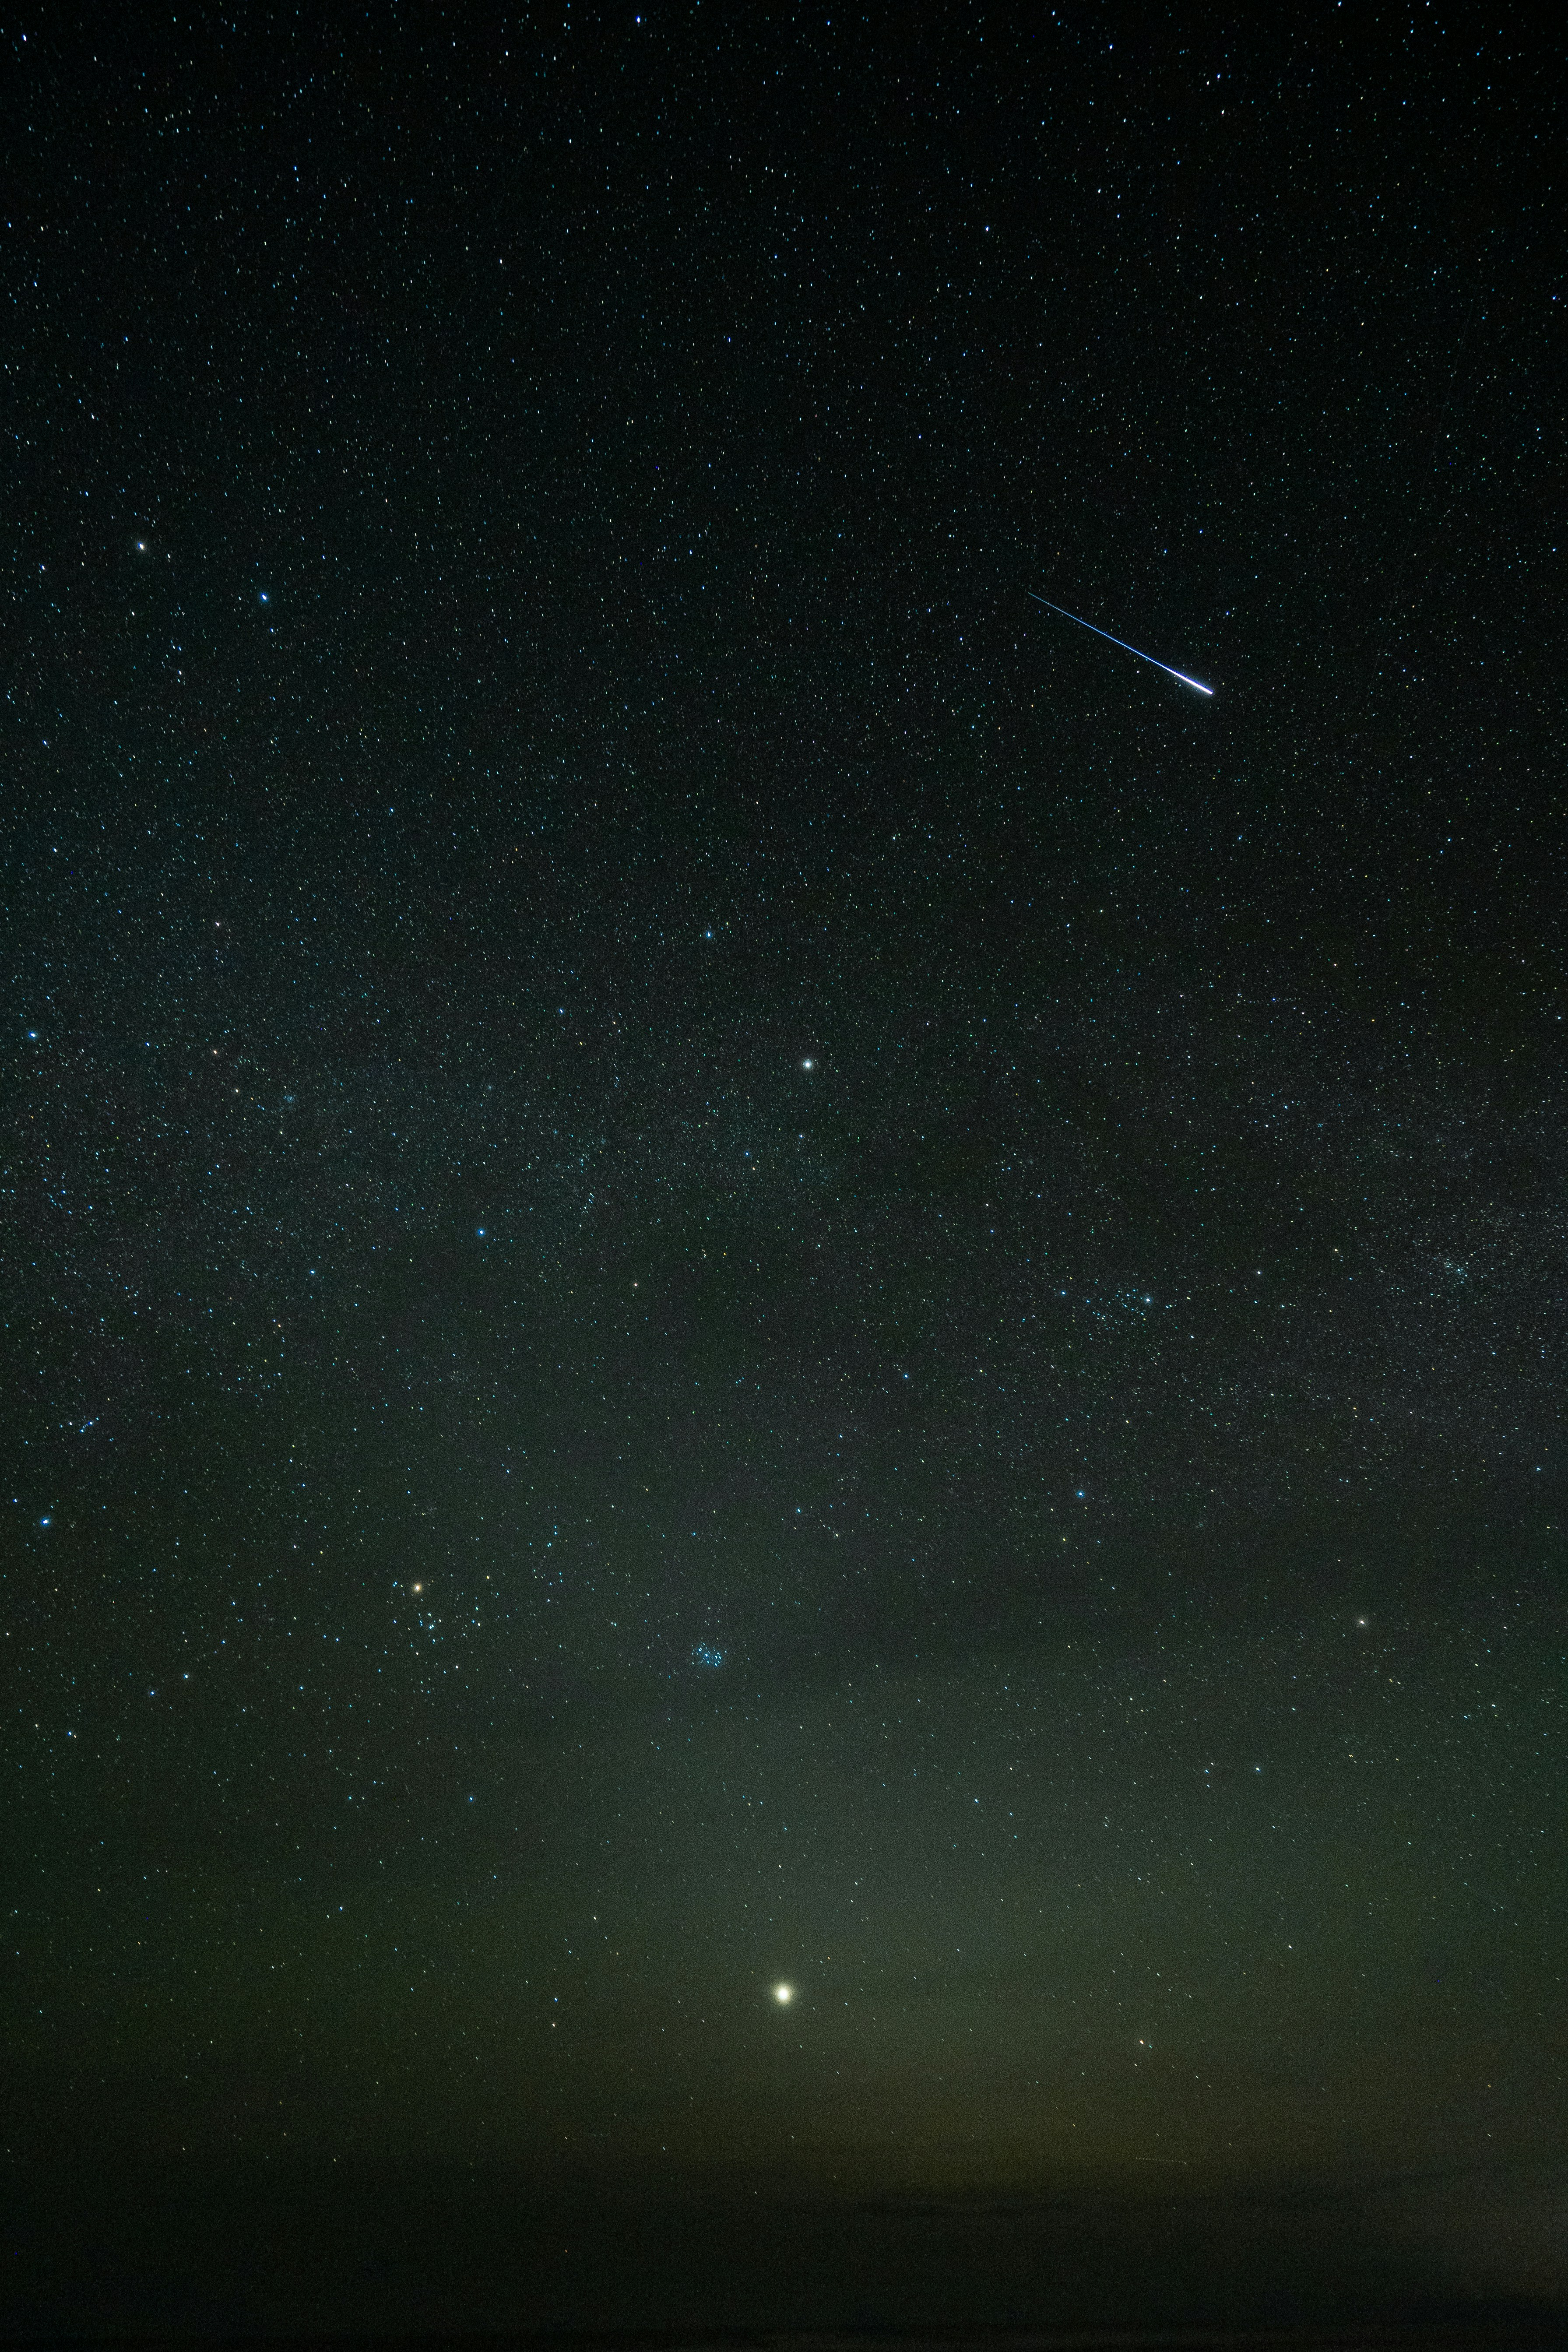
\includegraphics[width=0.5\linewidth]{P1.jpg}
		}%\hfill
		\subfloat{
			\includegraphics[width=0.5\linewidth]{P2.jpg}
		}\\
		\captionsetup{font=footnotesize}
		\bicaption{一些有关图片的描述。}{Some descriptions of the pictures in question.}
		\label{图:幂律参数空间}
	\end{figure}
	汤出,见野张网四面,祝曰:“自天下四方皆入吾网。”汤曰:“嘻,尽之矣!”乃去其三面,祝曰:“欲左,左。欲右,右。不用命,乃入吾网。”诸侯闻之,曰:“汤德至矣,及禽兽。”
	
	当是时,夏桀为虐政淫荒,而诸侯昆吾氏为乱。汤乃兴师率诸侯,伊尹从汤,汤自把钺以伐昆吾,遂伐桀。汤曰:“格女众庶,来,女悉听朕言。匪台小子敢行举乱,有夏多罪,予维闻女众言,夏氏有罪。予畏上帝,不敢不正。今夏多罪,天命殛之。今女有众,女曰:‘我君不恤我众,舍我啬事而割政’。女其曰:‘有罪,其奈何’?夏王率止众力,率夺夏国。众有率怠不和,曰:‘是日何时丧?予与女皆亡’!夏德若兹,今朕必往。尔尚及予一人致天之罚,予其大理女。女毋不信,朕不食言。女不从誓言,予则帑僇女,无有攸赦。”以告令师,作汤誓。於是汤曰:“吾甚武”,号曰武王。
	
	桀败於有娀之虚,桀奔於鸣条,夏师败绩。汤遂伐三嵕,俘厥宝玉,义伯、仲伯作典宝。汤既胜夏,欲迁其社,不可,作夏社。伊尹报。於是诸侯毕服,汤乃践天子位,平定海内。
	
	汤归至于泰卷陶,中垒作诰。既绌夏命,还亳,作汤诰:“维三月,王自至於东郊。告诸侯群后:‘毋不有功於民,勤力乃事。予乃大罚殛女,毋予怨。’曰:‘古禹、皋陶久劳于外,其有功乎民,民乃有安。东为江,北为济,西为河,南为淮,四渎已修,万民乃有居。后稷降播,农殖百谷。三公咸有功于民,故後有立。昔蚩尤与其大夫作乱百姓,帝乃弗予,有状。先王言不可不勉。’曰:‘不道,毋之在国,女毋我怨。’”以令诸侯。伊尹作咸有一德,咎单作明居。
	
	汤乃改正朔,易服色,上白,朝会以昼。
	
	汤崩,太子太丁未立而卒,於是乃立太丁之弟外丙,是为帝外丙。帝外丙即位三年,崩,立外丙之弟中壬,是为帝中壬。帝中壬即位四年,崩,伊尹乃立太丁之子太甲。太甲,成汤适长孙也,是为帝太甲。帝太甲元年,伊尹作伊训,作肆命,作徂后。
	
	帝太甲既立三年,不明,暴虐,不遵汤法,乱德,於是伊尹放之於桐宫。三年,伊尹摄行政当国,以朝诸侯。
	
	帝太甲居桐宫三年,悔过自责,反善,於是伊尹乃迎帝太甲而授之政。帝太甲修德,诸侯咸归殷,百姓以宁。伊尹嘉之,乃作太甲训三篇,褒帝太甲,称太宗。
	
	太宗崩,子沃丁立。帝沃丁之时,伊尹卒。既葬伊尹於亳,咎单遂训伊尹事,作沃丁。
	
	沃丁崩,弟太庚立,是为帝太庚。帝太庚崩,子帝小甲立。帝小甲崩,弟雍己立,是为帝雍己。殷道衰,诸侯或不至。
	
	帝雍己崩,弟太戊立,是为帝太戊。帝太戊立伊陟为相。亳有祥桑谷共生於朝,一暮大拱。帝太戊惧,问伊陟。伊陟曰:“臣闻妖不胜德,帝之政其有阙与?帝其修德。”太戊从之,而祥桑枯死而去。伊陟赞言于巫咸。巫咸治王家有成,作咸艾,作太戊。帝太戊赞伊陟于庙,言弗臣,伊陟让,作原命。殷复兴,诸侯归之,故称中宗。
	% Please add the following required packages to your document preamble:
	% \usepackage{booktabs}
	\begin{table}[htb]
		\centering
		\captionsetup{font=footnotesize}
		\bicaption{符号对照表}{Symbol cross-reference table}
		\label{表:符号对照表}
		\begin{tabular}{@{}cc@{}}
			\toprule
			符号          & 含义                                                              \\ \midrule
			$a$         & 尺度因子                                                            \\
			$k$         & 波尔兹曼常数                                                          \\
			$T_c$       & 一些描述                                                   \\
			$t_c$       & 一些描述                                                   \\
			$\beta$     & 一些描述                                           \\
			$t_b$       & 仍然是一些描述                                                        \\ \bottomrule
		\end{tabular}
	\end{table}
	中宗崩,子帝中丁立。帝中丁迁于隞。河亶甲居相。祖乙迁于邢。帝中丁崩,弟外壬立,是为帝外壬。仲丁书阙不具。帝外壬崩,弟河亶甲立,是为帝河亶甲。河亶甲时,殷复衰。
	
	河亶甲崩,子帝祖乙立。帝祖乙立,殷复兴。巫贤任职。
	
	祖乙崩,子帝祖辛立。帝祖辛崩,弟沃甲立,是为帝沃甲。帝沃甲崩,立沃甲兄祖辛之子祖丁,是为帝祖丁。帝祖丁崩,立弟沃甲之子南庚,是为帝南庚。帝南庚崩,立帝祖丁之子阳甲,是为帝阳甲。帝阳甲之时,殷衰。
	
	自中丁以来,废適而更立诸弟子,弟子或争相代立,比九世乱,於是诸侯莫朝。
	
	帝阳甲崩,弟盘庚立,是为帝盘庚。帝盘庚之时,殷已都河北,盘庚渡河南,复居成汤之故居,乃五迁,无定处。殷民咨胥皆怨,不欲徙。盘庚乃告谕诸侯大臣曰:“昔高后成汤与尔之先祖俱定天下,法则可修。舍而弗勉,何以成德!”乃遂涉河南,治亳,行汤之政,然後百姓由宁,殷道复兴。诸侯来朝,以其遵成汤之德也。
	
	帝盘庚崩,弟小辛立,是为帝小辛。帝小辛立,殷复衰。百姓思盘庚,乃作盘庚三篇。帝小辛崩,弟小乙立,是为帝小乙。
	
	帝小乙崩,子帝武丁立。帝武丁即位,思复兴殷,而未得其佐。三年不言,政事决定於冢宰,以观国风。武丁夜梦得圣人,名曰说。以梦所见视群臣百吏,皆非也。於是乃使百工营求之野,得说於傅险中。是时说为胥靡,筑於傅险。见於武丁,武丁曰是也。得而与之语,果圣人,举以为相,殷国大治。故遂以傅险姓之,号曰傅说。
		
	帝武丁祭成汤,明日,有飞雉登鼎耳而呴,武丁惧。祖己曰:“王勿忧,先修政事。”祖己乃训王曰:“唯天监下典厥义,降年有永有不永,非天夭民,中绝其命。民有不若德,不听罪,天既附命正厥德,乃曰其奈何。鸣呼!王嗣敬民,罔非天继,常祀毋礼于弃道。”武丁修政行德,天下咸驩,殷道复兴。
	
	帝武丁崩,子帝祖庚立。祖己嘉武丁之以祥雉为德,立其庙为高宗,遂作高宗肜日及训。
	
	帝祖庚崩,弟祖甲立,是为帝甲。帝甲淫乱,殷复衰。
	
	帝甲崩,子帝廪辛立。帝廪辛崩,弟庚丁立,是为帝庚丁。帝庚丁崩,子帝武乙立。殷复去亳,徙河北。
	
	帝武乙无道,为偶人,谓之天神。与之博,令人为行。天神不胜,乃僇辱之。为革囊,盛血,昂而射之,命曰“射天”。武乙猎於河渭之闲,暴雷,武乙震死。子帝太丁立。帝太丁崩,子帝乙立。帝乙立,殷益衰。
	
	帝乙长子曰微子启,启母贱,不得嗣。少子辛,辛母正后,辛为嗣。帝乙崩,子辛立,是为帝辛,天下谓之纣。
	
	帝纣资辨捷疾,闻见甚敏;材力过人,手格猛兽;知足以距谏,言足以饰非;矜人臣以能,高天下以声,以为皆出己之下。好酒淫乐,嬖於妇人。爱妲己,妲己之言是从。於是使师涓作新淫声,北里之舞,靡靡之乐。厚赋税以实鹿台之钱,而盈钜桥之粟。益收狗马奇物,充仞宫室。益广沙丘苑台,多取野兽蜚鸟置其中。慢於鬼神。大聚乐戏於沙丘,以酒为池,县肉为林,使男女裸相逐其间,为长夜之饮。
	
	百姓怨望而诸侯有畔者,於是纣乃重刑辟,有炮格之法。以西伯昌、九侯、鄂侯为三公。九侯有好女,入之纣。九侯女不喜淫,纣怒,杀之,而醢九侯。鄂侯争之彊,辨之疾,并脯鄂侯。西伯昌闻之,窃叹。崇侯虎知之,以告纣,纣囚西伯羑里。西伯之臣闳夭之徒,求美女奇物善马以献纣,纣乃赦西伯。西伯出而献洛西之地,以请除炮格之刑。纣乃许之,赐弓矢斧钺,使得征伐,为西伯。而用费中为政。费中善谀,好利,殷人弗亲。纣又用恶来。恶来善毁谗,诸侯以此益疏。
	
	西伯归,乃阴修德行善,诸侯多叛纣而往归西伯。西伯滋大,纣由是稍失权重。王子比干谏,弗听。商容贤者,百姓爱之,纣废之。及西伯伐饥国,灭之,纣之臣祖伊闻之而咎周,恐,奔告纣曰:“天既讫我殷命,假人元龟,无敢知吉,非先王不相我後人,维王淫虐用自绝,故天弃我,不有安食,不虞知天性,不迪率典。今我民罔不欲丧,曰‘天曷不降威,大命胡不至’?今王其柰何?”纣曰:“我生不有命在天乎!”祖伊反,曰:“纣不可谏矣。”西伯既卒,周武王之东伐,至盟津,诸侯叛殷会周者八百。诸侯皆曰:“纣可伐矣。”武王曰:“尔未知天命。”乃复归。
	
	纣愈淫乱不止。微子数谏不听,乃与大师、少师谋,遂去。比干曰:“为人臣者,不得不以死争。”乃彊谏纣。纣怒曰:“吾闻圣人心有七窍。”剖比干,观其心。箕子惧,乃详狂为奴,纣又囚之。殷之大师、少师乃持其祭乐器奔周。周武王於是遂率诸侯伐纣。纣亦发兵距之牧野。甲子日,纣兵败。纣走入,登鹿台,衣其宝玉衣,赴火而死。周武王遂斩纣头,县之[大]白旗。杀妲己。释箕子之囚,封比干之墓,表商容之闾。封纣子武庚、禄父,以续殷祀,令修行盘庚之政。殷民大说。於是周武王为天子。其後世贬帝号,号为王。而封殷后为诸侯,属周。
	
	周武王崩,武庚与管叔、蔡叔作乱,成王命周公诛之,而立微子於宋,以续殷后焉。
	
	太史公曰:余以颂次契之事,自成汤以来,采於书诗。契为子姓,其後分封,以国为姓,有殷氏、来氏、宋氏、空桐氏、稚氏、北殷氏、目夷氏。孔子曰,殷路车为善,而色尚白。
	
	
	\pagebreak
	{\zihao{5}\bibliography{References,PBHEMF,MagneticMonopoles}}%这里的References,PBHEMF,MagneticMonopoles均是bib文件,如果只有一个文件那就只写一个,有多个就写多个,英文逗号隔开
	\pagebreak
	
	\begin{appendices}
%		\appendix
		\setcounter{table}{0}
		\setcounter{figure}{0}
		\setcounter{equation}{0}
		\renewcommand{\thetable}{\thesection-\arabic{table}}
		\renewcommand{\theequation}{\thesection-\arabic{equation}}
		\renewcommand{\thefigure}{\thesection-\arabic{figure}}
		
		\ctexset{section={name={附录},number=\thesection}}%修改章节序号以符合附录
		
		
		
		\section{第一个附录\label{附录:第一个附录}}
		周后稷,名弃。其母有邰氏女,曰姜原。姜原为帝喾元妃。姜原出野,见巨人迹,心忻然说,欲践之,践之而身动如孕者。居期而生子,以为不祥,弃之隘巷,马牛过者皆辟不践;徙置之林中,適会山林多人,迁之;而弃渠中冰上,飞鸟以其翼覆荐之。姜原以为神,遂收养长之。初欲弃之,因名曰弃。
		
		弃为兒时,屹如巨人之志。其游戏,好种树麻、菽,麻、菽美。及为成人,遂好耕农,相地之宜,宜穀者稼穑焉,民皆法则之。帝尧闻之,举弃为农师,天下得其利,有功。帝舜曰:“弃,黎民始饥,尔后稷播时百穀。”封弃於邰,号曰后稷,别姓姬氏。后稷之兴,在陶唐、虞、夏之际,皆有令德。
		
		后稷卒,子不窋立。不窋末年,夏后氏政衰,去稷不务,不窋以失其官而饹戎狄之间。不窋卒,子鞠立。鞠卒,子公刘立。公刘虽在戎狄之间,复脩后稷之业,务耕种,行地宜,自漆、沮度渭,取材用,行者有资,居者有畜积,民赖其庆。百姓怀之,多徙而保归焉。周道之兴自此始,故诗人歌乐思其德。公刘卒,子庆节立,国於豳。
		
		庆节卒,子皇仆立。皇仆卒,子差弗立。差弗卒,子毁隃立。毁隃卒,子公非立。公非卒,子高圉立。高圉卒,子亚圉立。亚圉卒,子公叔祖类立。公叔祖类卒,子古公亶父立。古公亶父复脩后稷、公刘之业,积德行义,国人皆戴之。薰育戎狄攻之,欲得财物,予之。已复攻,欲得地与民。民皆怒,欲战。古公曰:“有民立君,将以利之。今戎狄所为攻战,以吾地与民。民之在我,与其在彼,何异。民欲以我故战,杀人父子而君之,予不忍为。”乃与私属遂去豳,度漆、沮,逾梁山,止於岐下。豳人举国扶老携弱,尽复归古公於岐下。及他旁国闻古公仁,亦多归之。於是古公乃贬戎狄之俗,而营筑城郭室屋,而邑别居之。作五官有司。民皆歌乐之,颂其德。
		
		古公有长子曰太伯,次曰虞仲。太姜生少子季?,季历娶太任,皆贤妇人,生昌,有圣瑞。古公曰:“我世当有兴者,其在昌乎?”长子太伯、虞仲知古公欲立季历以传昌,乃二人亡如荆蛮,文身断发,以让季历。
		
		古公卒,季历立,是为公季。公季脩古公遗道,笃於行义,诸侯顺之。
		
		公季卒,子昌立,是为西伯。西伯曰文王,遵后稷、公刘之业,则古公、公季之法,笃仁,敬老,慈少。礼下贤者,日中不暇食以待士,士以此多归之。伯夷、叔齐在孤竹,闻西伯善养老,盍往归之。太颠、闳夭、散宜生、鬻子、辛甲大夫之徒皆往归之。
		
		\pagebreak %强制结束此页,也可以使用\newpage代替
		
		\section{第二个附录\label{附录:第二个附录}}
		崇侯虎谮西伯於殷纣曰:“西伯积善累德,诸侯皆向之,将不利於帝。”帝纣乃囚西伯於羑里。闳夭之徒患之。乃求有莘氏美女,骊戎之文马,有熊九驷,他奇怪物,因殷嬖臣费仲而献之纣。纣大说,曰:“此一物足以释西伯,况其多乎!”乃赦西伯,赐之弓矢斧钺,使西伯得征伐。曰:“谮西伯者,崇侯虎也。”西伯乃献洛西之地,以请纣去砲格之刑。纣许之。
		
		西伯阴行善,诸侯皆来决平。於是虞、芮之人有狱不能决,乃如周。入界,耕者皆让畔,民俗皆让长。虞、芮之人未见西伯,皆惭,相谓曰:“吾所争,周人所耻,何往为,祇取辱耳。”遂还,俱让而去。诸侯闻之,曰“西伯盖受命之君”。
		
		明年,伐犬戎。明年,伐密须。明年,败耆国。殷之祖伊闻之,惧,以告帝纣。纣曰:“不有天命乎?是何能为!”明年,伐邘。明年,伐崇侯虎。而作丰邑,自岐下而徙都丰。明年,西伯崩,太子发立,是为武王。
		
		西伯盖即位五十年。其囚羑里,盖益易之八卦为六十四卦。诗人道西伯,盖受命之年称王而断虞芮之讼。後十年而崩,谥为文王。改法度,制正朔矣。追尊古公为太王,公季为王季:盖王瑞自太王兴。
		
		武王即位,太公望为师,周公旦为辅,召公、毕公之徒左右王,师脩文王绪业。
		
		九年,武王上祭于毕。东观兵,至于盟津。为文王木主,载以车,中军。武王自称太子发,言奉文王以伐,不敢自专。乃告司马、司徒、司空、诸节:“齐栗,信哉!予无知,以先祖有德臣,小子受先功,毕立赏罚,以定其功。”遂兴师。师尚父号曰:“总尔众庶,与尔舟楫,後至者斩。”武王渡河,中流,白鱼跃入王舟中,武王俯取以祭。既渡,有火自上复于下,至于王屋,流为乌,其色赤,其声魄云。是时,诸侯不期而会盟津者八百诸侯。诸侯皆曰:“纣可伐矣。”武王曰:“女未知天命,未可也。”乃还师归。
		
		居二年,闻纣昏乱暴虐滋甚,杀王子比干,囚箕子。太师疵、少师彊抱其乐器而饹周。於是武王遍告诸侯曰:“殷有重罪,不可以不毕伐。”乃遵文王,遂率戎车三百乘,虎贲三千人,甲士四万五千人,以东伐纣。十一年十二月戊午,师毕渡盟津,诸侯咸会。曰:“孳孳无怠!”武王乃作太誓,告于众庶:“今殷王纣乃用其妇人之言,自绝于天,毁坏其三正,离逷其王父母弟,乃断弃其先祖之乐,乃为淫声,用变乱正声,怡说妇人。故今予发维共行天罚。勉哉夫子,不可再,不可三!”
		\pagebreak
	\end{appendices}
	

	\section*{攻读学位期间发表论文与研究成果清单}\addcontentsline{toc}{section}{攻读学位期间发表论文与研究成果清单}

	\noindent[1]\ Wang X Z, Deng C M. The primordial black holes solution to the cosmological monopole problem[J]. The European Physical Journal C, 2024, 84(1): 31.
	\pagebreak
	\section*{致谢}\addcontentsline{toc}{section}{致谢}
	\fangsong
	感谢国家!
\end{document}